%\documentclass{article}
%\usepackage{graphicx,subfigure}
%\begin{document}

\begin{figure}[!hb]
  \centering
  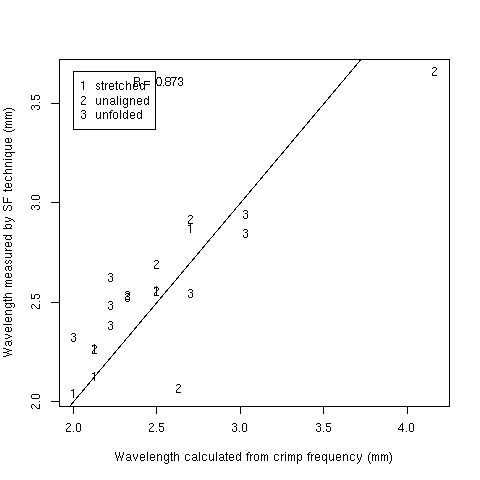
\includegraphics[width=1.0\textwidth]{figcrimpwavlsf.png}
%   crimpwavlsf.png is original 
  \caption{Correlation between wavelength calculated from staple crimp frequency and wavelength measured by the SF technique}
  \label{fig:crimpwavlsf}
\end{figure}

%\end{document}

